\documentclass{standalone}
\usepackage{amsmath}
\usepackage{tikz}

\begin{document}
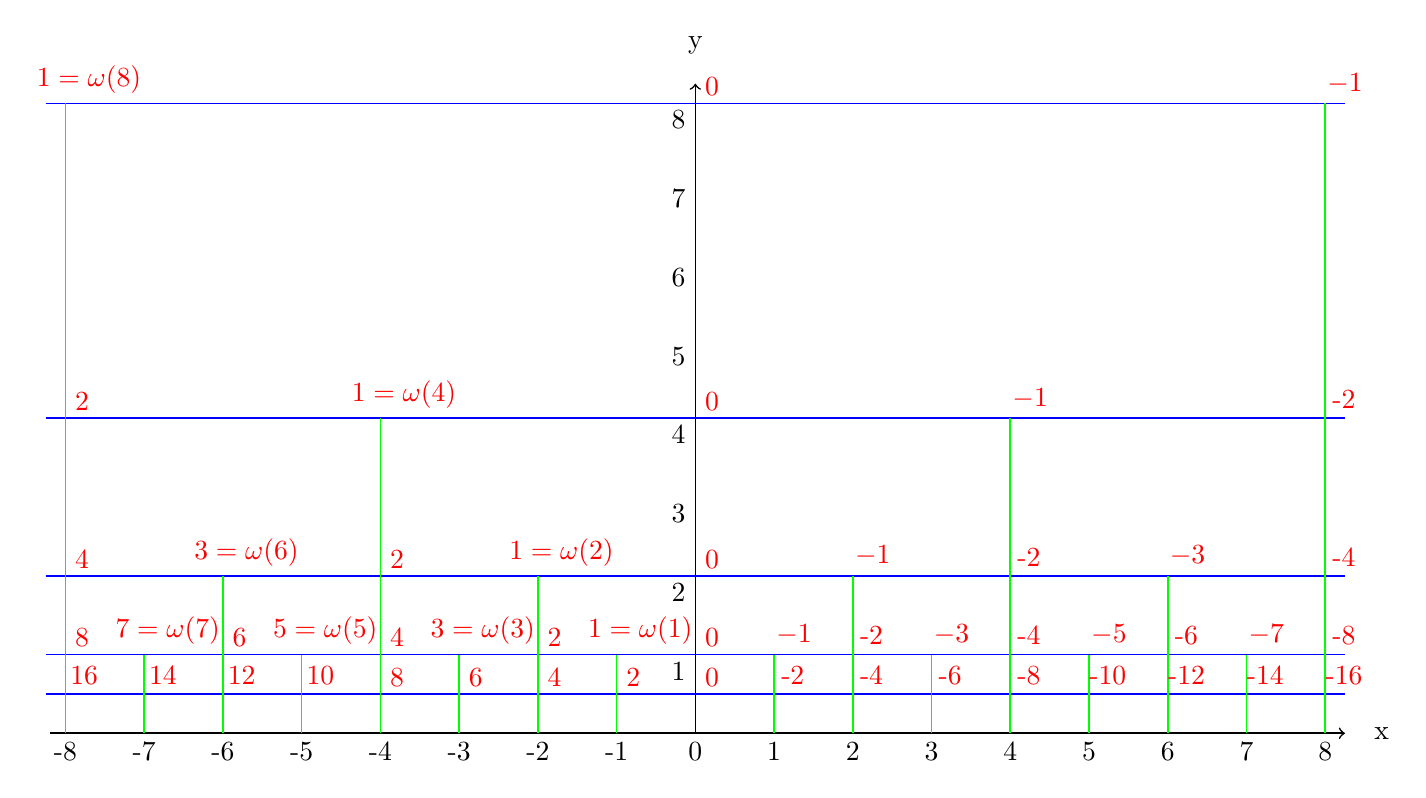
\begin{tikzpicture}
\draw [black, line width=0.6pt, ->] (0,0) to[out=90,in=270] (0,8.25);
\node [anchor=south] at (0,8.5) {y};
\draw [black, line width=0.6pt, ->] (-8.2,0) to[out=0,in=180] (8.25,0);
\node [anchor=west] at (8.5,0) {x};
\foreach \x in {-8,-7,-6,-5,-4,-3,-2,-1,0,1,2,3,4,5,6,7,8}
  \node [anchor=north] at (\x,0) {\x};
\foreach \y in {1,2,3,4,5,6,7,8}
  \node [anchor=45] at (0,\y) {\y};

\draw [blue, line width=0.6pt] (-8.25,0.5) to[out=0,in=180] (8.25,0.5);
\draw [blue, line width=0.6pt] (-8.25,1) to[out=0,in=180] (8.25,1);
\draw [blue, line width=0.6pt] (-8.25,2) to[out=0,in=180] (8.25,2);
\draw [blue, line width=0.6pt] (-8.25,4) to[out=0,in=180] (8.25,4);
\draw [blue, line width=0.6pt] (-8.25,8) to[out=0,in=180] (8.25,8);

\draw [green, line width=0.6pt] (-8,0) to[out=90,in=270] (-8,1);
\draw [green, line width=0.6pt] (-7,0) to[out=90,in=270] (-7,1);
\draw [green, line width=0.6pt] (-6,0) to[out=90,in=270] (-6,1);
\draw [green, line width=0.6pt] (-5,0) to[out=90,in=270] (-5,1);
\draw [green, line width=0.6pt] (-4,0) to[out=90,in=270] (-4,1);
\draw [green, line width=0.6pt] (-3,0) to[out=90,in=270] (-3,1);
\draw [green, line width=0.6pt] (-2,0) to[out=90,in=270] (-2,1);
\draw [green, line width=0.6pt] (-1,0) to[out=90,in=270] (-1,1);
\draw [green, line width=0.6pt] (1,0) to[out=90,in=270] (1,1);
\draw [green, line width=0.6pt] (2,0) to[out=90,in=270] (2,1);
\draw [green, line width=0.6pt] (3,0) to[out=90,in=270] (3,1);
\draw [green, line width=0.6pt] (4,0) to[out=90,in=270] (4,1);
\draw [green, line width=0.6pt] (5,0) to[out=90,in=270] (5,1);
\draw [green, line width=0.6pt] (6,0) to[out=90,in=270] (6,1);
\draw [green, line width=0.6pt] (7,0) to[out=90,in=270] (7,1);
\draw [green, line width=0.6pt] (8,0) to[out=90,in=270] (8,1);

\draw [green, line width=0.6pt] (-8,1) to[out=90,in=270] (-8,2);
\draw [green, line width=0.6pt] (-6,1) to[out=90,in=270] (-6,2);
\draw [green, line width=0.6pt] (-4,1) to[out=90,in=270] (-4,2);
\draw [green, line width=0.6pt] (-2,1) to[out=90,in=270] (-2,2);
\draw [green, line width=0.6pt] (2,1) to[out=90,in=270] (2,2);
\draw [green, line width=0.6pt] (4,1) to[out=90,in=270] (4,2);
\draw [green, line width=0.6pt] (6,1) to[out=90,in=270] (6,2);
\draw [green, line width=0.6pt] (8,1) to[out=90,in=270] (8,2);

\draw [green, line width=0.6pt] (-8,2) to[out=90,in=270] (-8,4);
\draw [green, line width=0.6pt] (-4,2) to[out=90,in=270] (-4,4);
\draw [green, line width=0.6pt] (4,2) to[out=90,in=270] (4,4);
\draw [green, line width=0.6pt] (8,2) to[out=90,in=270] (8,4);

\draw [green, line width=0.6pt] (-8,4) to[out=90,in=270] (-8,8);
\draw [green, line width=0.6pt] (8,4) to[out=90,in=270] (8,8);

\node [anchor=225, red] at (-8,0.5) {16};
\node [anchor=225, red] at (-7,0.5) {14};
\node [anchor=225, red] at (-6,0.5) {12};
\node [anchor=225, red] at (-5,0.5) {10};
\node [anchor=225, red] at (-4,0.5) {8};
\node [anchor=225, red] at (-3,0.5) {6};
\node [anchor=225, red] at (-2,0.5) {4};
\node [anchor=225, red] at (-1,0.5) {2};
\node [anchor=225, red] at (0,0.5) {0};
\node [anchor=225, red] at (1,0.5) {-2};
\node [anchor=225, red] at (2,0.5) {-4};
\node [anchor=225, red] at (3,0.5) {-6};
\node [anchor=225, red] at (4,0.5) {-8};
\node [anchor=225, red] at (5,0.5) {-10};
\node [anchor=225, red] at (6,0.5) {-12};
\node [anchor=225, red] at (7,0.5) {-14};
\node [anchor=225, red] at (8,0.5) {-16};

\node [anchor=225, red] at (-8,1) {8};
\node [anchor=225, red] at (-7,1) {$7 = \omega(7)$};
\node [anchor=225, red] at (-6,1) {6};
\node [anchor=225, red] at (-5,1) {$5 = \omega(5)$};
\node [anchor=225, red] at (-4,1) {4};
\node [anchor=225, red] at (-3,1) {$3 = \omega(3)$};
\node [anchor=225, red] at (-2,1) {2};
\node [anchor=225, red] at (-1,1) {$1 = \omega(1)$};
\node [anchor=225, red] at (0,1) {0};
\node [anchor=225, red] at (1,1) {$-1$};
\node [anchor=225, red] at (2,1) {-2};
\node [anchor=225, red] at (3,1) {$-3$};
\node [anchor=225, red] at (4,1) {-4};
\node [anchor=225, red] at (5,1) {$-5$};
\node [anchor=225, red] at (6,1) {-6};
\node [anchor=225, red] at (7,1) {$-7$};
\node [anchor=225, red] at (8,1) {-8};

\node [anchor=225, red] at (-8,2) {4};
\node [anchor=225, red] at (-6,2) {$3 = \omega(6)$};
\node [anchor=225, red] at (-4,2) {2};
\node [anchor=225, red] at (-2,2) {$1 = \omega(2)$};
\node [anchor=225, red] at (0,2) {0};
\node [anchor=225, red] at (2,2) {$-1$};
\node [anchor=225, red] at (4,2) {-2};
\node [anchor=225, red] at (6,2) {$-3$};
\node [anchor=225, red] at (8,2) {-4};

\node [anchor=225, red] at (-8,4) {2};
\node [anchor=225, red] at (-4,4) {$1 = \omega(4)$};
\node [anchor=225, red] at (0,4) {0};
\node [anchor=225, red] at (4,4) {$-1$};
\node [anchor=225, red] at (8,4) {-2};

\node [anchor=225, red] at (-8,8) {$1 = \omega(8)$};
\node [anchor=225, red] at (0,8) {0};
\node [anchor=225, red] at (8,8) {$-1$};

\end{tikzpicture}
\end{document}
